\section{Introduction to HPC and Its View from R}
\makesubcontentsslides

\subsection{An R and \protect\pbdR View of Parallel Hardware and Software}
\makesubcontentsslidessec

\begin{frame}{R Interfaces to Low-Level Native Tools}
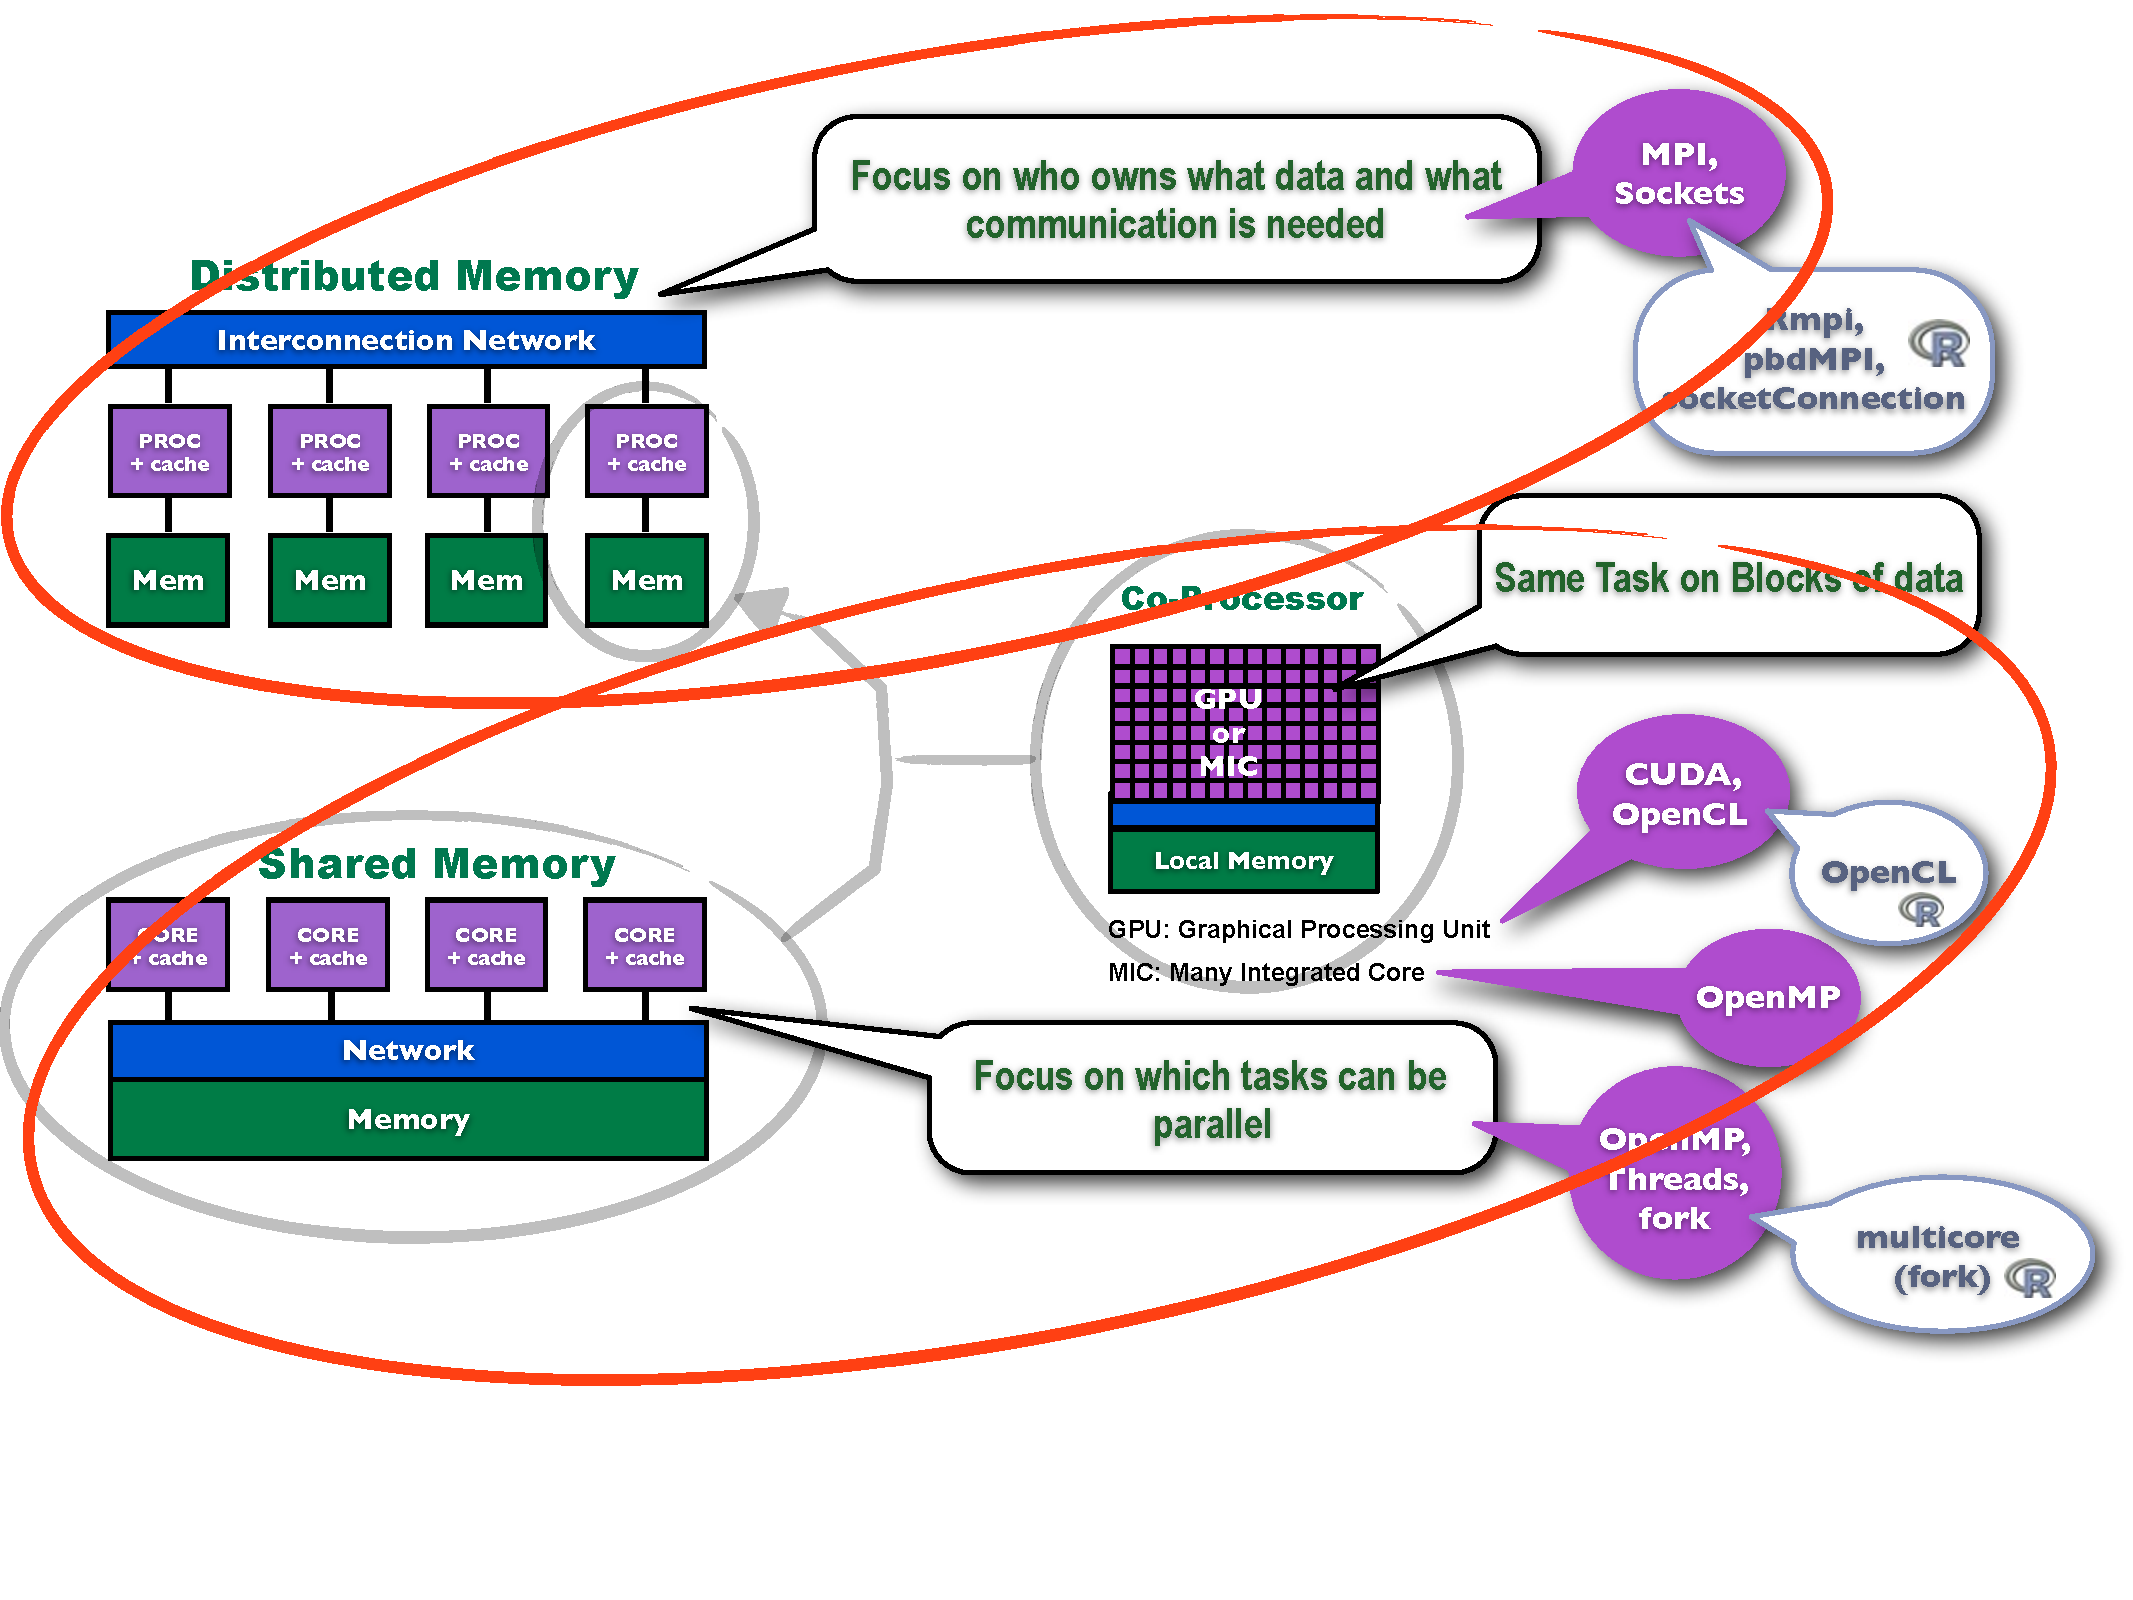
\includegraphics[height=\textheight]
{../common/pics/hardware/ParallelHardware10.pdf}
\end{frame}

\begin{frame}{HPC Libraries: 30+ Years of Research}
\includegraphics[height=\textheight]
{../common/pics/hardware/ParallelHardware25.pdf}
\end{frame}

\begin{frame}{R and \pbdR R Interfaces to HPC Libraries}
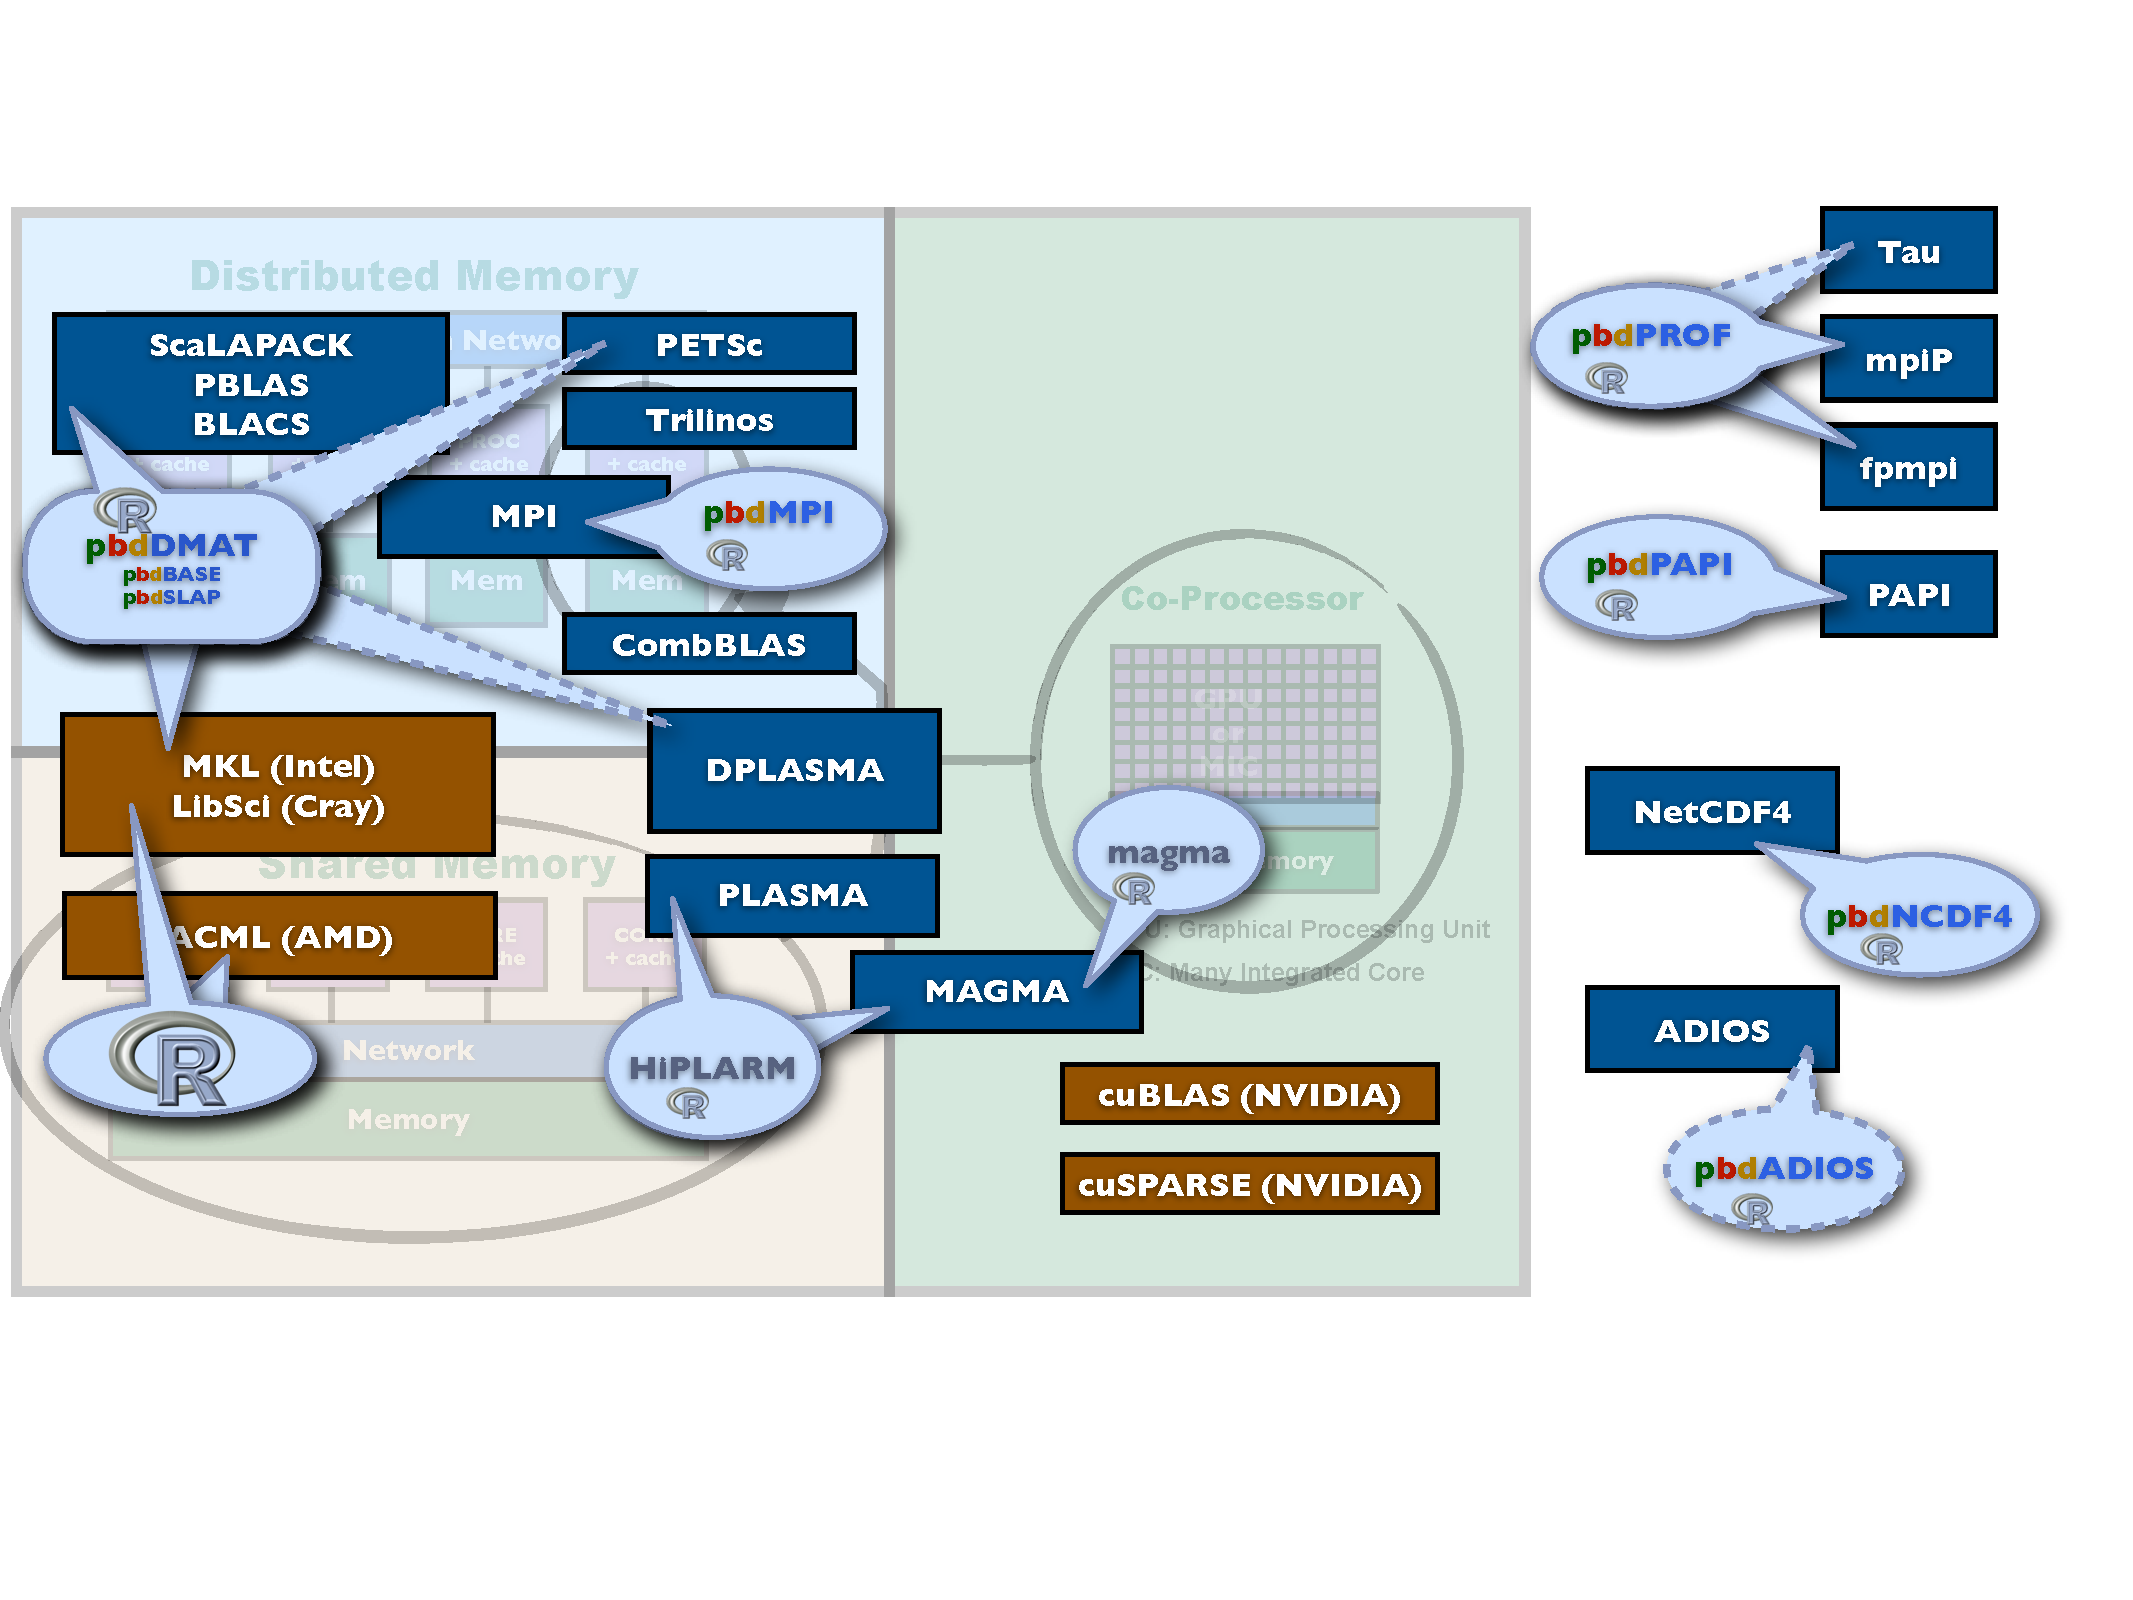
\includegraphics[height=\textheight]
{../common/pics/hardware/ParallelHardware26.pdf}
\end{frame}

\begin{frame}{Big Data and Little Data}
\begin{minipage}{10cm}
  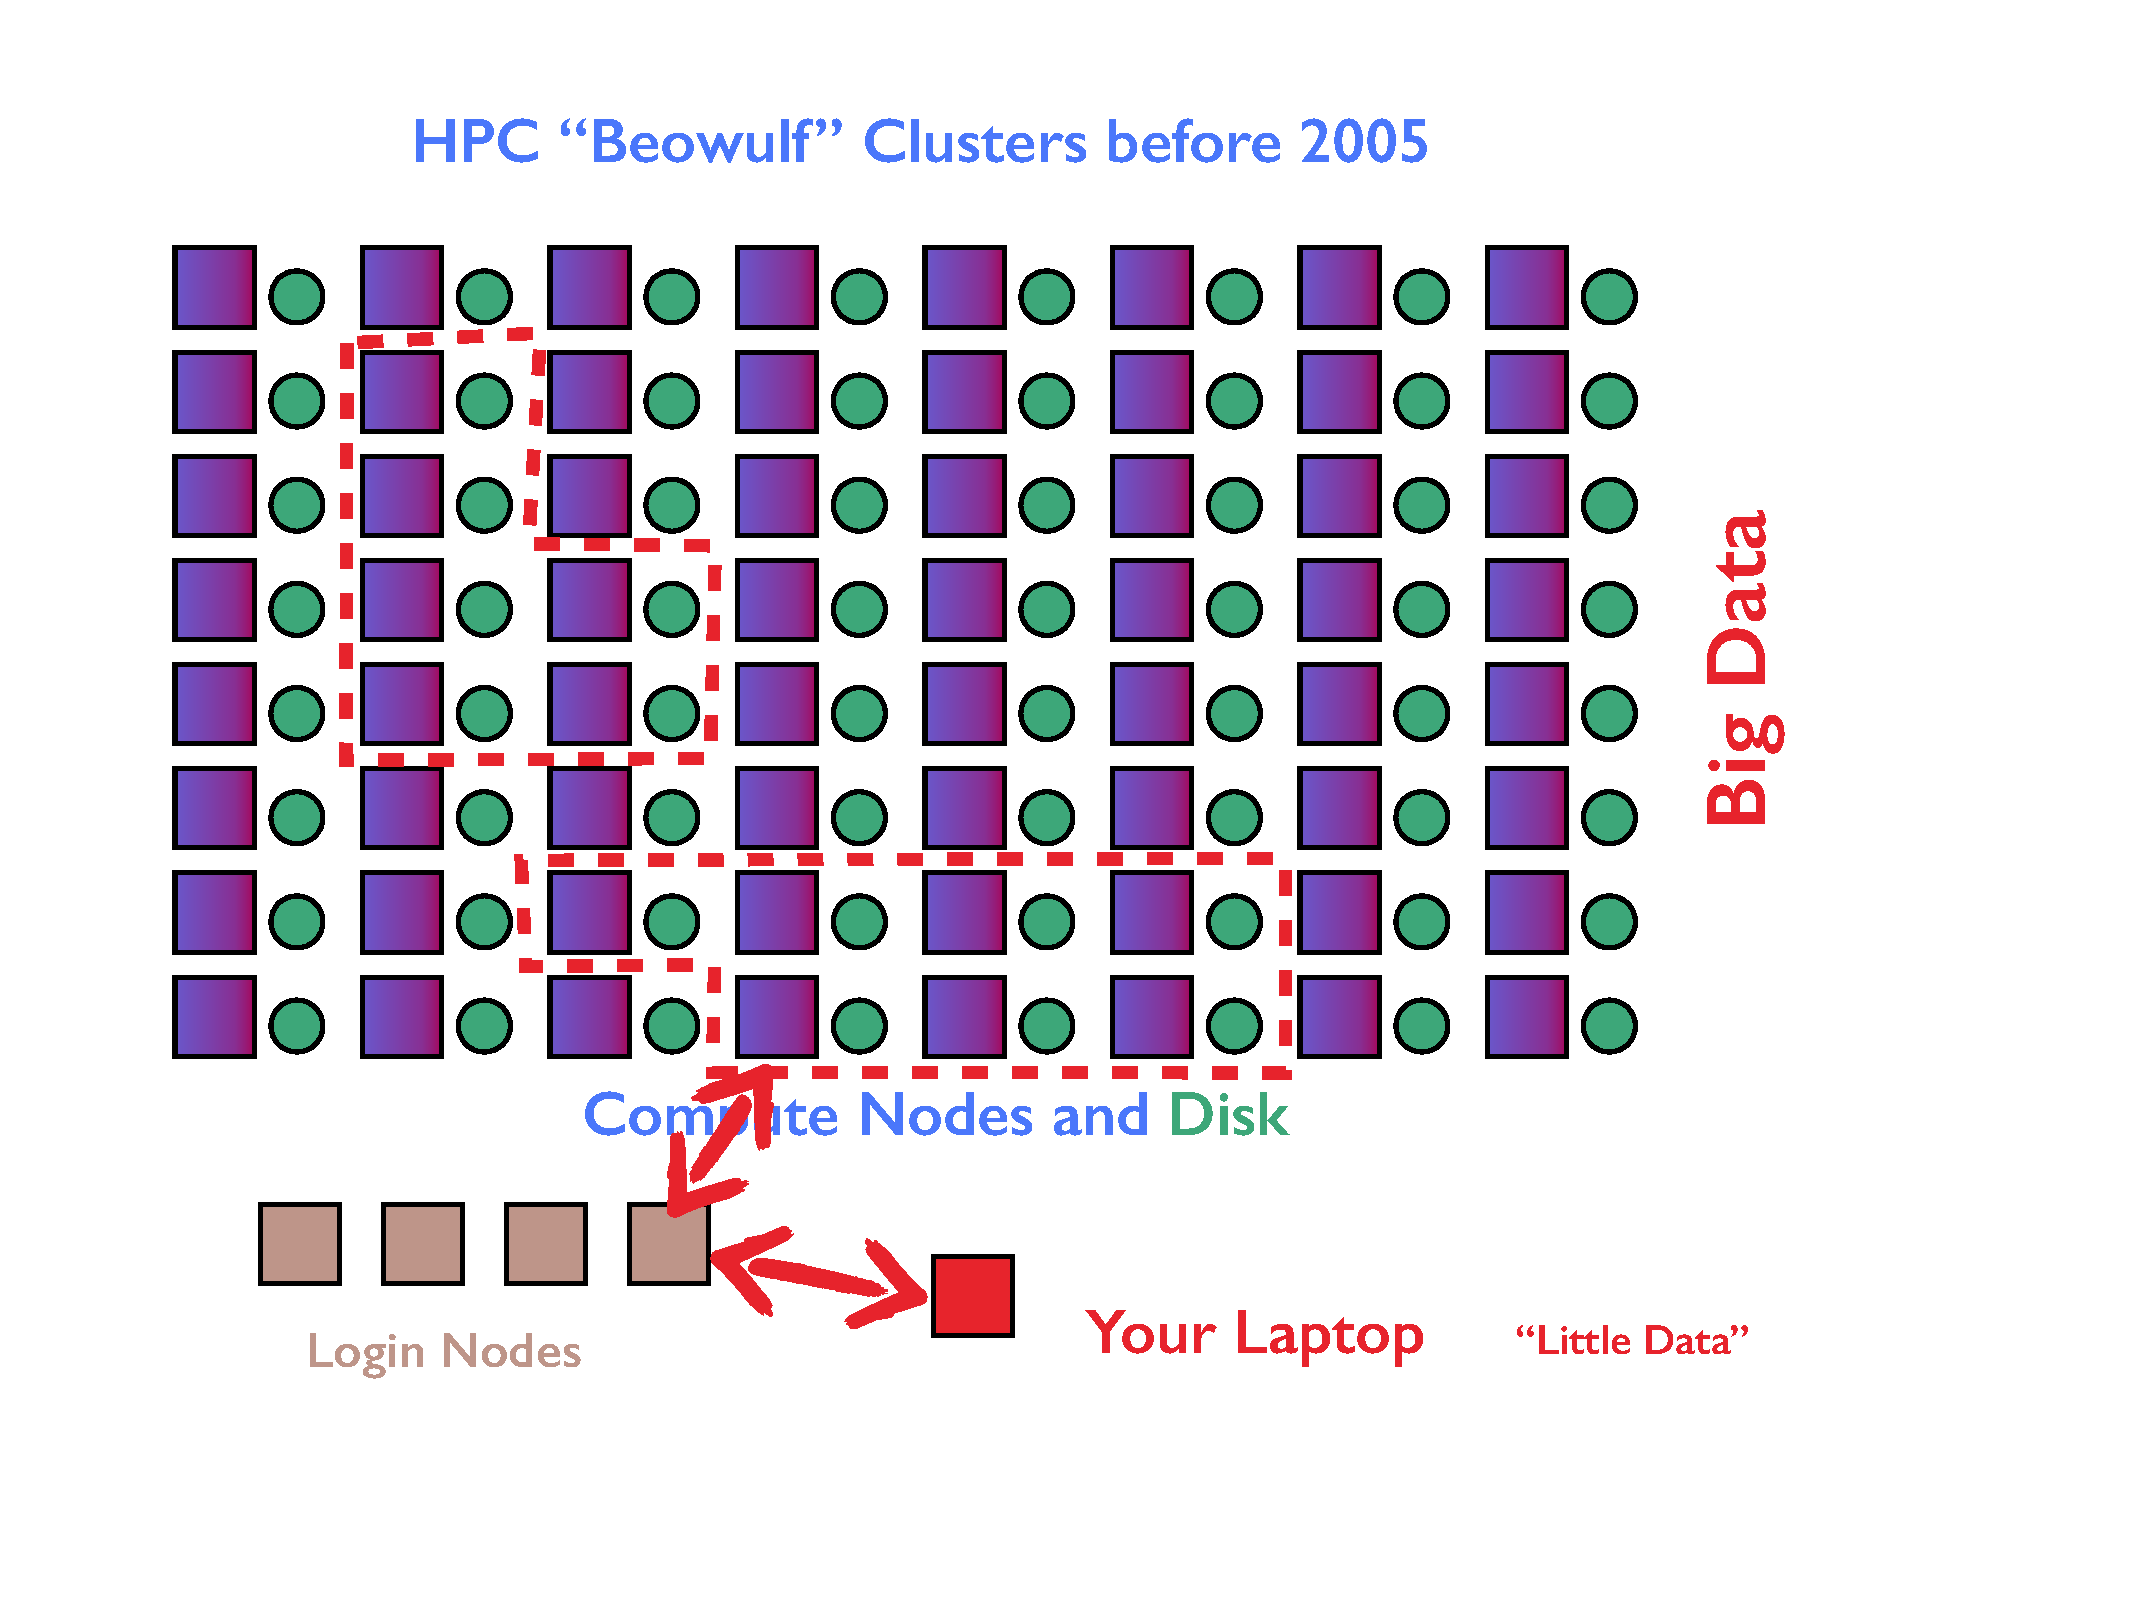
\includegraphics[height=0.9\textheight]
  {../common/pics/hardware/ParallelHardware22.pdf}\hfill
\end{minipage}
\begin{minipage}{5cm}\small
  \begin{block}{Analysis Workflow}\pause
    \begin{itemize}[<+-|alert@+>]
    \item Get Big Data
      \begin{itemize}
      \item Parallel data reader
      \item Parallel data generator
      \end{itemize}
    \item Write analysis script
    \item Graphics to display results
    \item Profile and optimize code
    \end{itemize}
  \end{block}
\end{minipage}
\end{frame}

\begin{frame}{Hadoop: Will it merge with HPC in the future?}
\begin{minipage}{8.5cm}
  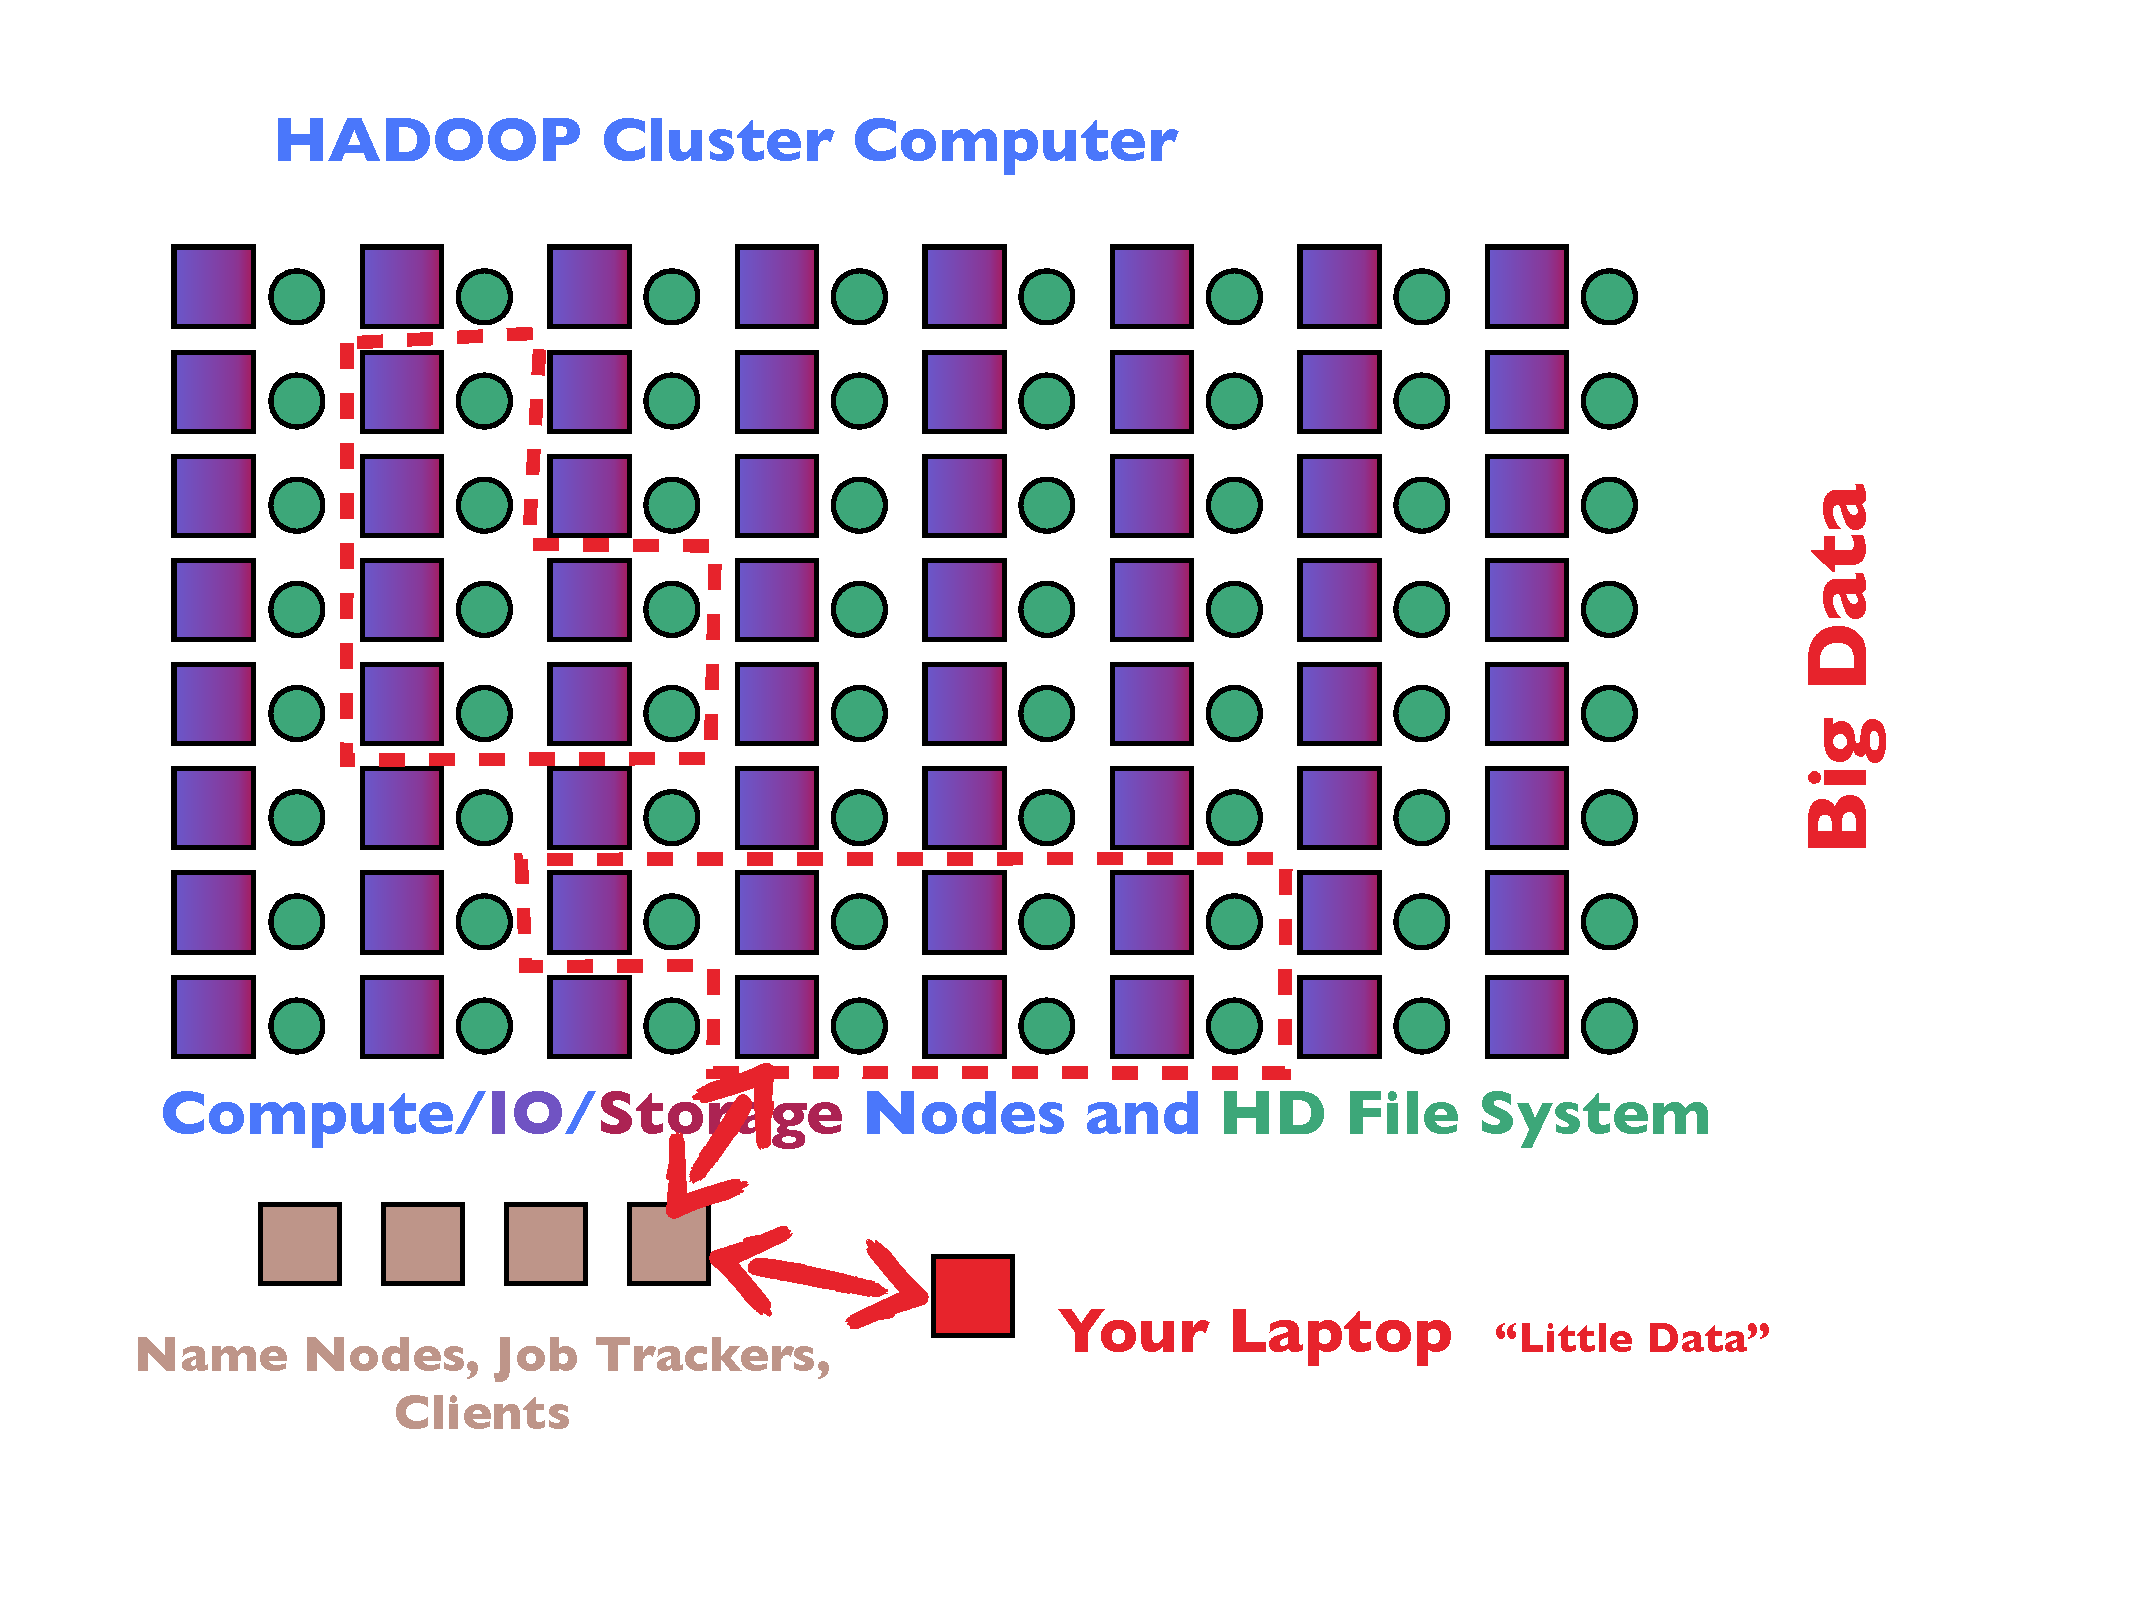
\includegraphics[trim=2cm 0cm 0cm 0cm,clip=true,height=0.8\textheight]
  {../common/pics/hardware/ParallelHardware23.pdf}
\end{minipage}
\begin{minipage}{3cm}\small
  \begin{block}{Components}\pause
%    \begin{itemize}[<+-|alert@+>]
    \scriptsize HDFS file system\\
    Yarn resource manager \\
    Map-reduce limitation
%    \end{itemize}
  \end{block}
\end{minipage}
\end{frame}

\begin{frame}{The future is here}
\includegraphics[height=0.9\textheight]
{../common/pics/hardware/ParallelHardware24.pdf}
\end{frame}

%\begin{frame}{\pbdR Interfaces to Libraries: Sustainable Path}
%\includegraphics[height=1.05\textheight]
%{../common/pics/hardware/ParallelHardware14.pdf}
%\end{frame}

%\begin{frame}{Low level R Interfaces to Native Tools}
%\includegraphics[width=0.95\textheight]
%{../common/pics/hardware/ParallelHardware22.pdf}
%\includegraphics[width=0.95\textheight]
%{../common/pics/hardware/ParallelHardware23.pdf}
%\end{frame}



\subsection{Batch and Interactive}
\makesubcontentsslidessec

\begin{frame}
  \begin{block}{Data analysis is interactive!}
    \pause
    \begin{itemize}[<+-|alert@+>]
    \item Data reduction to knowledge
    \item Iterative process with same data
      \begin{itemize}
      \item Exploration, model construction
      \item Diagnostics of fit and quantification of uncertainty
      \item Interpretation
      \end{itemize}
    \item S (and R) interactive ``answer'' to batch data analysis
    \item Efficient use of expensive people
    \end{itemize}
  \end{block}
  \begin{block}{Big platform computing is batch!}
    \pause
    \begin{itemize}[<+-|alert@+>]
    \item Libraries built for batch computing
    \item Traditionally data generation by simulation science
    \item Efficient use of expensive platforms
    \end{itemize}
  \end{block}
\end{frame}

\begin{frame}
  \begin{block}{High-Level Language: Batch and Interactive Distinction Blurred.}
    \begin{itemize}
    \item A function is a ``batch'' script
    \item \R ``An interactive environment to use batch scripts''
    \end{itemize}
  \end{block}
  \begin{block}{Ideal solution: Interactive Client with a Batch
      Server}
    \begin{itemize}
    \item Parallel visualization systems (VisIt and ParaView) are
      client-server (batch on server)
    \item Current \pbdR packages address server side (batch)
    \item pbdCS 0.1-0 released on GitHub
      \begin{itemize}
      \item Interactive SPMD
      \item Based on ZeroMQ distributed messaging (pbdZMQ 0.1-1 on CRAN)
      \item Bridge resource manager (pbdSCHED 0.1-0 on GitHub)
      \item Site configuration file
      \item Manage relationship of big data (server side) to little
        data (client side)
      \end{itemize}
    \end{itemize}
  \end{block}
\end{frame}


\subsection{Programming Models}
\makesubcontentsslidessec

\begin{frame}{Manager-Workers}
  \begin{block}{}
    \begin{itemize}
    \item A serial program (Manager) divides up work and/or data
    \item Workers run in parallel without interaction
    \item Manager collects/combines results from workers
    \item Divide-Recombine fits this model
    \end{itemize}
  \end{block}
\end{frame}

\begin{frame}{MapReduce}
  \begin{block}{}
    \begin{itemize}
    \item A concept born of a search engine
    \item Decouples certain coupled problems with an intermediate
      communication - shuffle
    \item User writes two serial codes: Map and Reduce
    \end{itemize}
  \end{block}
\end{frame}

\begin{frame}{MapReduce: a Parallel Search Engine Concept}
  \begin{block}{Search MANY documents \hfill Serve MANY users}
    \begin{center}\scriptsize
      \begin{equation*}
        \begin{array}{c@{\hspace{-2ex}}r@{\hspace{-2ex}}c}
          \begin{array}{c}
            \mbox{\scriptsize Web} \\
            \mbox{\scriptsize Pages} \\
            \mbox{\scriptsize (records)}
          \end{array} &
          \begin{array}{c}\tiny
            \\ \mbox{\tiny p0} \\ \mbox{\tiny p1} \\
            \mbox{\tiny p2} \\ \mbox{\tiny p3}
          \end{array} &
          \begin{array}{c}
            \mbox{\scriptsize Index Words (keys)} \\
            \left[
            \begin{array}{cccc}
              A_1 & A_2  & A_3 & A_4 \\
              \hline
              B_1 & B_2  & B_3 & B_4 \\
              \hline
              C_1 & C_2  & C_3 & C_4 \\
              \hline
              D_1 & D_2  & D_3 & D_4
            \end{array}
            \right]
          \end{array}
        \end{array}
        \hbox{\hspace{-2ex}}
        \begin{array}{c}
          \hbox{Shuffle} \\
          \longrightarrow \\
          \mbox{\code{MPI\_Alltoallv}}
        \end{array}
        \hbox{\hspace{-2ex}}
        \begin{array}{c@{\hspace{-2ex}}r@{\hspace{-2ex}}c}
          \begin{array}{c}
            \mbox{\scriptsize Index} \\
            \mbox{\scriptsize Words} \\
            \mbox{\scriptsize (keys)}
          \end{array} &
          \begin{array}{c}
            \\  \mbox{\tiny p0} \\ \mbox{\tiny p1} \\
            \mbox{\tiny p2} \\ \mbox{\tiny p3}
          \end{array} &
          \begin{array}{c}
            \mbox{\scriptsize Web Pages (records)} \\
            \left[
            \begin{array}{cccc}
              A_1 & B_1  & C_1 & D_1 \\
              \hline
              A_2 & B_2  & C_2 & D_2 \\
              \hline
              A_3 & B_3  & C_3 & D_3 \\
              \hline
              A_4 & B_4  & C_4 & D_4
            \end{array}
            \right]
          \end{array}
        \end{array}
      \end{equation*}
    \end{center}
    \vspace{2em}
    \begin{center}
      Matrix transpose in another language?
    \end{center}
  \end{block}
\end{frame}

\begin{frame}
  \begin{block}{Can use different sets of processors}
    \begin{center}
      \begin{equation*}\scriptsize
        \begin{array}{c@{\hspace{-2ex}}r@{\hspace{-2ex}}c}
          \begin{array}{c}
            \mbox{\scriptsize Web} \\
            \mbox{\scriptsize Pages} \\
            \mbox{\scriptsize (records)}
          \end{array} &
          \begin{array}{c}\tiny
            \\ \mbox{\tiny p0} \\ \mbox{\tiny p1} \\
            \mbox{\tiny p2} \\ \mbox{\tiny p3}
          \end{array} &
          \begin{array}{c}
            \mbox{\scriptsize Index Words (keys)} \\
            \left[
            \begin{array}{cccc}
              \\
              \hline
              B_1 & B_2  & B_3 & B_4 \\
              \hline
              \\
              \hline
              \\
            \end{array}
            \right]
          \end{array}
        \end{array}
        \hbox{\hspace{-2ex}}
        \begin{array}{c}
          \hbox{Streaming} \\
          \hbox{Shuffle} \\
          \longrightarrow \\
          \mbox{\code{MPI\_Scatter}}
        \end{array}
        \hbox{\hspace{-2ex}}
        \begin{array}{c@{\hspace{-2ex}}r@{\hspace{-2ex}}c}
          \begin{array}{c}
            \mbox{\scriptsize Index} \\
            \mbox{\scriptsize Words} \\
            \mbox{\scriptsize (keys)}
          \end{array} &
          \begin{array}{c}
            \\  \mbox{\tiny p4} \\ \mbox{\tiny p5} \\
            \mbox{\tiny p6} \\ \mbox{\tiny p7}
          \end{array} &
          \begin{array}{c}
            \mbox{\scriptsize Web Pages (records)} \\
            \left[
            \begin{array}{cccc}
              \quad  & B_1  & \quad & \quad \\
              \hline
              \quad  & B_2  & \quad  &  \quad \\
              \hline
              \quad  & B_3  & \quad  &  \quad \\
              \hline
              \quad  & B_4  & \quad  & \quad
            \end{array}
            \right]
          \end{array}
        \end{array}
      \end{equation*}
    \end{center}
  \end{block}
\end{frame}

\begin{frame}{MPI and MapReduce}
  \begin{block}{Both Concepts are about Communication}
    \begin{itemize}
    \item One makes communication explicit, gives choices
    \item The other hides communication, uses one choice (shuffle)
    \end{itemize}
  \end{block}
\end{frame}

\begin{frame}{SPMD: Single Program Multiple Data}
  \begin{block}{}
    \begin{itemize}
    \item The prevalent way of distributed programming
    \item Can handle tightly coupled parallel computations
    \item It is designed for batch computing
    \item There is usually no manager - rather, all cooperate
    \item Prime driver behind MPI specification
    \end{itemize}
  \end{block}
\end{frame}

\begin{frame}{Early SPMD Work in Statistics: Crossproduct (Row-Block)}
  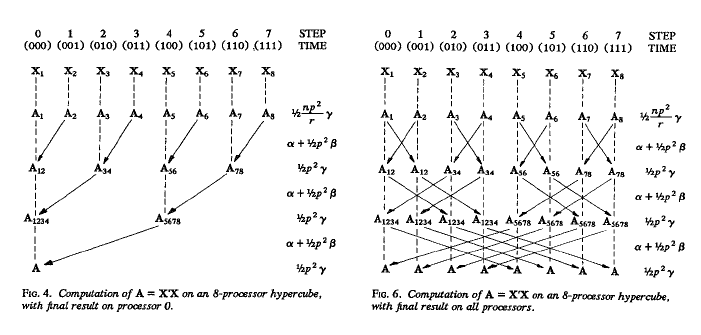
\includegraphics[width=\textwidth]
  {../common/pics/comm/Crossprod1987.png} \\
  \begin{block}{Hypercube: Individual send() and recv() over each dimension}
    {\scriptsize Ostrouchov (1987). Parallel Computing on a
      Hypercube: An overview of the architecture and some
      applications. {\em Proceedings of the 19th Symposium on the
        Interface of Computer Science and Statistics}, p.27-32.}
  \end{block}
\end{frame}

\begin{frame}{SPMD Simplified with MPI (and further with pbdMPI)}
  \includegraphics[trim=0cm 6cm 0cm 4cm,clip=true,width=\textwidth]
  {../common/pics/comm/ParallelHardware30.pdf}
  \vspace{-1ex}
  \begin{block}{Vendor MPI implementations: distributed + shared
      memory optimized}
    \begin{minipage}{4cm}
      \begin{itemize}
      \item \small Cray MPT
      \item \small SGI MPT
      \end{itemize}
    \end{minipage}
    \begin{minipage}{4cm}
      \begin{itemize}
      \item \small Intel MPI
      \end{itemize}
    \end{minipage}
  \end{block}
\end{frame}

\begin{frame}{Data-flow: Parallel Runtime Scheduling and Execution
    Controller (PaRSEC)}
  \vspace{-.1cm}
  \hspace{2cm}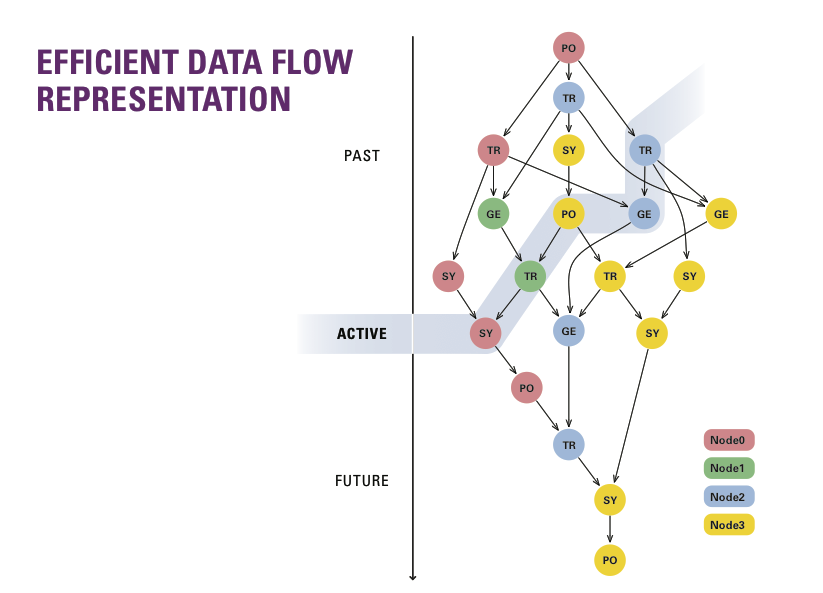
\includegraphics[trim=0cm 0cm 0cm
  1cm,clip=true,width=7.5cm]{../common/pics/comm/PaRSEC1.png}
 \\[-3.4cm]
  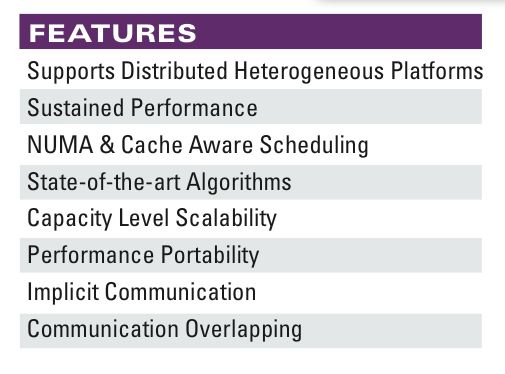
\includegraphics[width=4cm]{../common/pics/comm/PaRSEC2.png}
  \hspace{5cm}{\tiny Graphic from icl.cs.utk.edu}
  \begin{block}
    {\tiny Bosilca, G., Bouteiller, A., Danalis, A., Faverge,
      M., Herault, T., Dongarra, J. "PaRSEC: Exploiting Heterogeneity
      to Enhance Scalability," IEEE Computing in Science and
      Engineering, Vol. 15, No. 6, 36-45, November, 2013.}
    \begin{itemize}\small
    \item Master data-flow controller runs distributed on all cores.
    \item Dynamic generation of current level in flow graph
    \item Effectively removes collective synchronizations
    \end{itemize}
  \end{block}
\end{frame}
